%\subsection{Aplicativo}

\par Para iniciar o desenvolvimento do aplicativo, primeiramente fez-se
necessária a instalação e configuração da plataforma \textit{Android Studio}
versão 1.1.0 e \textit{Android SDK} versão 24.0.2.

	\par Logo após a configuração dos ambientes de desenvolvimento, o primeiro
passo foi a criação de uma \textit{activity main}, denominada
\textit{MainActivity}, a qual será executada quando a aplicação for iniciada. O
tipo de \textit{activity} escolhida é do tipo \textit{Navigation Drawer
Layout}. Na Figura \ref{fig:qm4}, pode-se ver o método
\texttt{onNavigationDrawerItemSelected()}, que tem por finalidade mostrar as
opções de navegação e o que deverá acontecer quando uma delas for clicada. Um
exemplo, caso o usuário escolha o item Notas, o software executará o
\textit{case} um, o qual criará uma \textit{intent} e chamará a classe
\texttt{ListaNotasActivity}.
	
		\begin{figure}[h!]
			\centerline{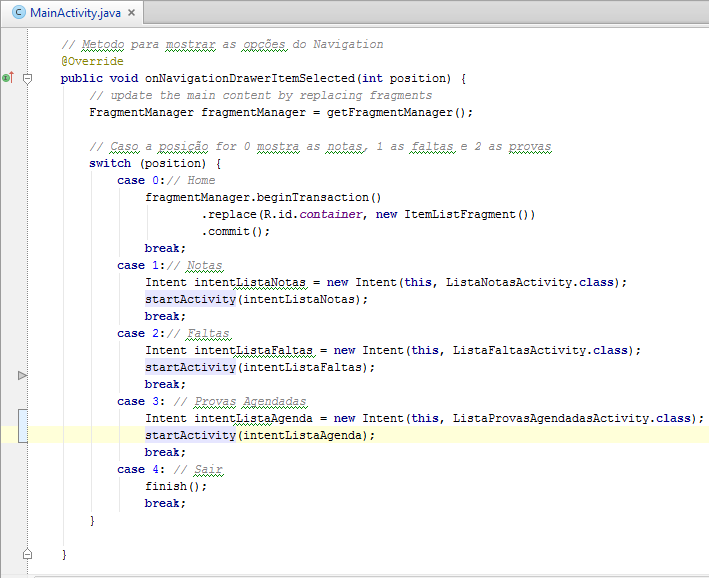
\includegraphics[scale=0.4]{./imagens/2_q_metodologico/qm4.png}}
			\caption[\textit{MainActivity}]{\textit{MainActivity}.
			 \textbf{Fonte:}Elaborado pelos autores.}
			\label{fig:qm4}
		\end{figure}
		\pagebreak
		
	\par O próximo passo, foi criar a \textit{activity Home}, o qual trará uma
lista de \textit{sites} uteis, com as opções Univás, MEC, Fies, Prouni e
\textit{Google} acadêmico. Para que essa lista aparecesse foi utilizada uma
\textit{activity} do tipo \textit{Master/Deital Flow} que já traz consigo o
\textit{widget} de \textit{ListView}. Na Figura \ref{fig:qm5}, pode-se ver a
classe \texttt{DummyContent}, local onde é declarado a lista de sites.
	
		
		\begin{figure}[h!]
			\centerline{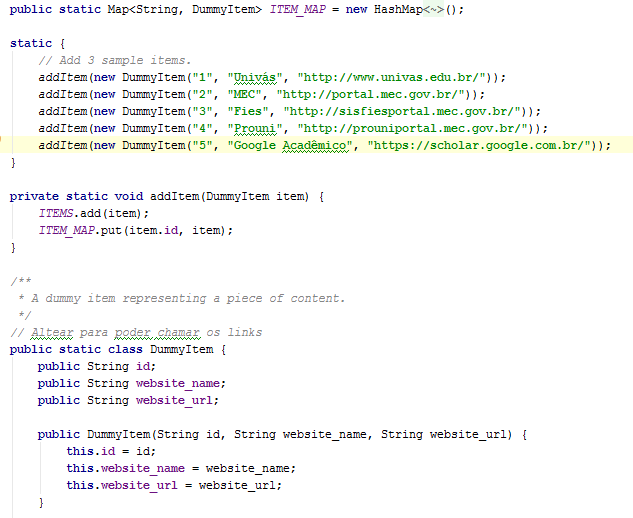
\includegraphics[scale=0.5]{./imagens/2_q_metodologico/qm5.png}}
			\caption[Classe \textit{DummyContent}]{Classe \textit{DummyContent}.
			 \textbf{Fonte:}Elaborado pelos autores.}
			\label{fig:qm5}
		\end{figure}

	\par Quando clicado em algum item, é executada a classe
\texttt{ItemDetailActivity}, que chamará o \texttt{ItemDetailFragment},
responsável por carregar o \textit{site} em questão no \textit{layout} do
aplicativo. Abaixo, na Figura \ref{fig:qm6}, vê-se o método responsável por
passar para o \textit{layout} o endereço do \textit{site}.
				
		\begin{figure}[h!]
			\centerline{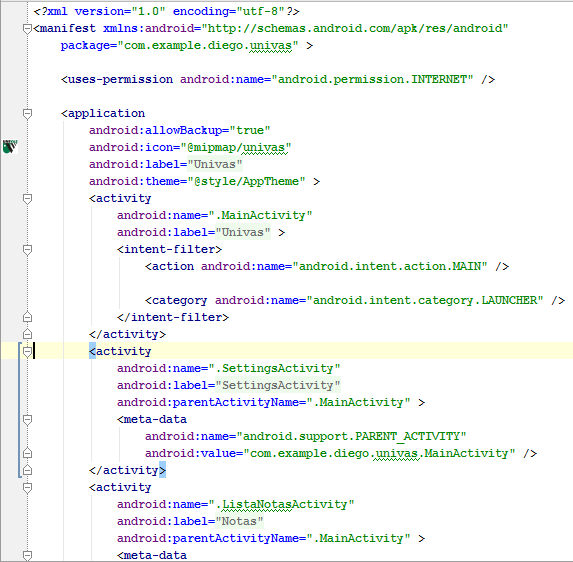
\includegraphics[scale=0.4]{./imagens/2_q_metodologico/qm6.png}}
			\caption[Método para carregar o \textit{layout} com \textit{web
			view}]{Método para carregar o \textit{layout} com \textit{web
			view}.
			 \textbf{Fonte:}Elaborado pelos autores.}
			\label{fig:qm6}
		\end{figure}

	\par Para que as informações possam aparecer, foram criadas
\textit{activities} do tipo \textit{Blank Activity}. No \textit{layout} dessas
\textit{activities} foram inseridas o \textit{widget ExpandableListView}, como
	é mostrado na Figura \ref{fig:qm7}.
	

		\begin{figure}[h!]
			\centerline{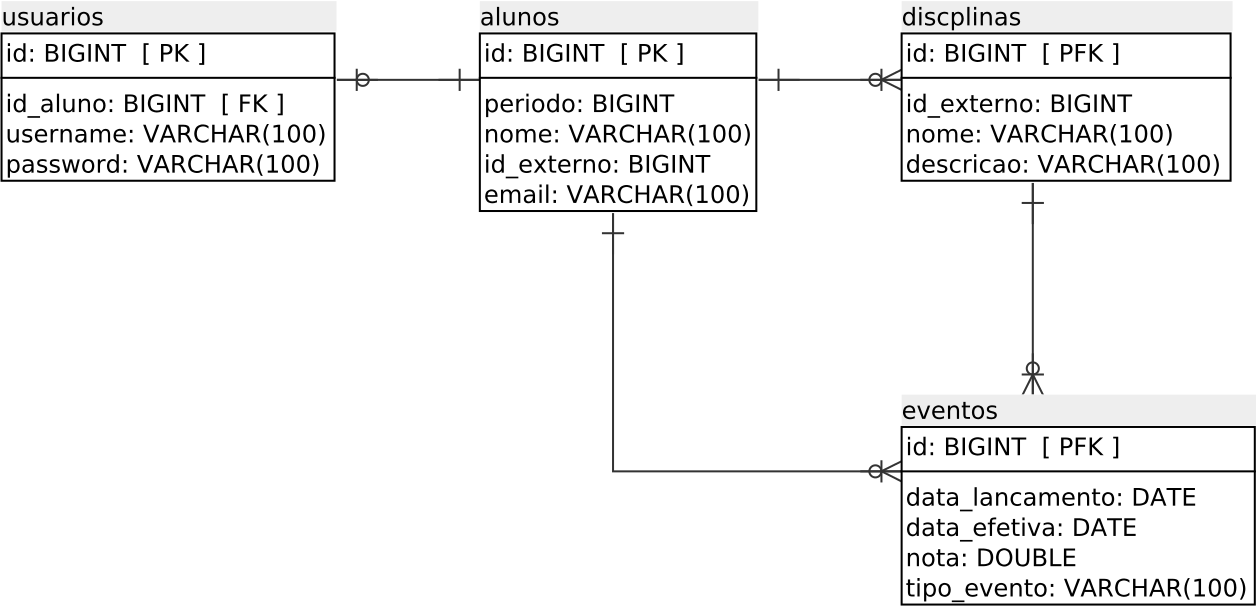
\includegraphics[scale=0.4]{./imagens/2_q_metodologico/qm7.png}}
			\caption[\textit{Layout} com \textit{expandable}]{\textit{Layout} com
			\textit{expandable}.
			 \textbf{Fonte:}Elaborado pelos autores.}
			\label{fig:qm7}
		\end{figure}		
		
	
		
%------------------------------------------------------------------------------
%------------------------------------------------------------------------------
%------------------------------------------------------------------------------
%------------------------------------------------------------------------------
%------------------------------------------------------------------------------
%------------------------------------------------------------------------------
		
	\par Foi criada uma classe chamada \texttt{BuscaDados}, que tem por finalidade
receber os dados do \textit{webservice}, salvá-los no banco de dados local do
aplicativo e entregá-los para as classes que implementam o \textit{Adapter}
para listar as informações na tela do dispositivo.
	
	\par No arquivo \texttt{AndroidManifest.xml} foi necessário alterar a opção
\texttt{Android:icon}, que define qual será o ícone do aplicativo. Por padrão,
ele apresenta o mascote do \textit{Android}, no entanto foi definida uma imagem
do logo da universidade. Foi necessário também incluir uma tag de
\texttt{uses-permission}, que obriga o usuário a permitir o uso da
\textit{internet} pelo aplicativo, conforme pode ser visto na Figura
\ref{fig:qm8}. Pode-se perceber que cada \textit{activity} encontra-se
dentro das tags \texttt{<activity><\/activity>} e que a \textit{activity main},
deve conter a tag \texttt{<intent-filter>} e dentro dela {\tiny{\texttt{<action
android:name="android.intent.action.MAIN" />}}}, indicando que
ela será a primeira a executar e {\tiny{\texttt{<category
android:name="android.intent.category.LAUNCHER" />}}}, informando que ficará
disponível junto aos outros aplicativos do dispositivo.
	
	\begin{figure}[h!]
			\centerline{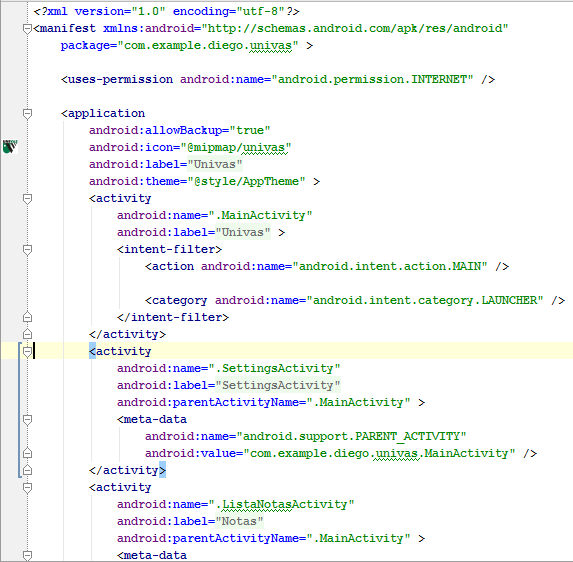
\includegraphics[scale=0.4]{./imagens/2_q_metodologico/qm8.png}}
			\caption[\texttt{AndroidManifest.xml}]{\texttt{AndroidManifest.xml}.
			 \textbf{Fonte:}Elaborado pelos autores.}
			\label{fig:qm8}
		\end{figure}
		\pagebreak

	\par O \textit{Android Studio} tem uma facilidade de se trabalhar com
controladores de versão, nesse caso foi escolhido o \textit{GitHub}. Nele foi
criada uma pasta e compartilhada entre os participantes e, por fim,
configurou-se o \textit{Git} com a IDE para que cada um possa ter a versão mais
atualizada do projeto.